%~~~~~~~~~~~~~~~~~~~~~~~~~~~~~~~~~~~~~~~~~~~~~~~~~~~~~~~~~~~~~~~~~~~~~
%    File      : prop_metodologia
%~~~~~~~~~~~~~~~~~~~~~~~~~~~~~~~~~~~~~~~~~~~~~~~~~~~~~~~~~~~~~~~~~~~~~

A metodologia utilizada para o desenvolvimento do projeto utilizará a técnica \MAIA\ (\maia) \cite{costa_um_2010}, cujo conceito simplificado é apresentado na \autoref{fig:maia}.

\begin{figure}[h]
  \centering
  \caption[\maia]{\MAIA\ -- \maia}\label{fig:maia}
  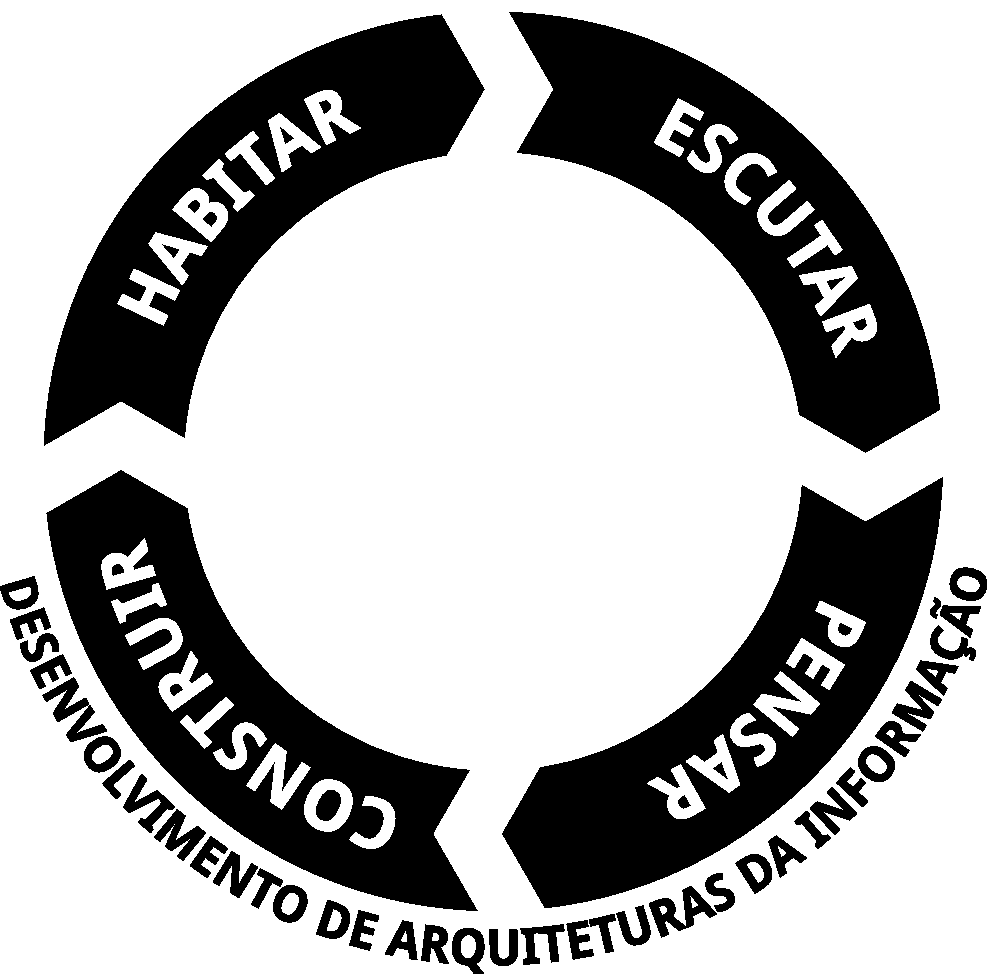
\includegraphics[width=0.4\linewidth,frame=0.5pt 5pt]{img/maia}
  \fonte{Equipe de pesquisa -- \textsc{cpai} (2016)}
\end{figure}

O Escutar, o Pensar, o Construir e o Habitar são momentos de atuação do sujeito sobre um espaço de informação. O Escutar e o Pensar são momentos voltados para os aspectos abstratos deste espaço. O Construir e o Habitar são momentos voltados para os aspectos concretos. O Escutar é o momento que concentra as percepções do espaço de informação. O Pensar concentra a modelagem hermenêutica de um espaço de informação. O Construir reúne as ações de manipulação dos elementos de um espaço de informação. O Habitar é o momento no qual o sujeito usa o espaço de informação percebido, modelado e aperfeiçoado com suas intenções. A configuração dos elementos em um espaço de informação é denominado de \AI (\siglaai).


\section{Instrumentos Metodológicos}\label{subsubsec:instrumentos_metodologicos}

A execução do projeto pressupõe que parte do conhecimento necessário para alcançar o resultado final será adquirido durante o próprio projeto. Isso acontece em razão de tratar-se de pesquisa aplicada, situação na qual a equipe de trabalho se propõe a fazer perguntas e descobrir respostas para as questões levantadas pelo problema a ser resolvido. Esse método de trabalho indica o uso de determinados instrumentos metodológicos que facilitam o levantamento e o aprofundamento dos temas a serem desenvolvidos no projeto, viabilizando uma abordagem colaborativa e mais focada no resultado final.


\section{Gestão do Projeto}\label{subsubsec:gestao_projeto}

Em função da complexidade do projeto e seus subprojetos, fica evidente a necessidade de uma camada de gestão para a coordenação científica, administrativa e operacional das diversas linhas de pesquisa e equipes de trabalho necessárias. A Gestão do Projeto trabalhará com modelos para assegurar a melhor alocação dos recursos financeiros e humanos necessários para alcançar os objetivos propostos, garantindo controle e segurança administrativa e jurídica durante todo o projeto.
